\subsection{Sources et Descriptions des données}
\subsubsection{Sources des données}
Les sources de données proviennent d'un entrepôt de données appelé RADIS qui regroupe toutes les données de l'université, notamment les données relatives aux étudiants, aux enseignants et aux ressources académiques.  
Pour accéder aux données, je me suis connecté avec les identifiants fournis par la division. Une fois connecté, j'ai effectué des requêtes via l'interface en ciblant les tables pertinentes.  
Les informations nécessaires ont été choisies en amont par la Division des Études Statistiques (DES) pour répondre aux besoins d'analyse.  
Enfin, les données ont été extraites au format CSV pour faciliter leur manipulation et analyse ultérieure.

\subsubsection{Description des données} 
Les données sont des données étudiants de plusieurs années couvrant une période allant de 2001 à 2025.  
Les données extraites comprennent plusieurs informations sur les étudiants, notamment :
\begin{itemize}
    \item \textbf{Identifiant étudiant} : Un identifiant unique pour chaque étudiant. 
    \item \textbf{INE Étudiant} : Un identifiant national étudiant (INE) unique pour chaque étudiant, utilisé pour l'identification officielle.
    \item \textbf{Nom et prénom, sexe} : Les noms, prénoms et le sexe des étudiants.
    \item \textbf{Date de naissance} : La date de naissance des étudiants.
    \item \textbf{Lieu et région de naissance} : Le lieu et la région de naissance de l'étudiant.
    \item \textbf{Faculté} : La faculté à laquelle l'étudiant est inscrit.
    \item \textbf{Département} : Le département spécifique au sein de la faculté.
    \item \textbf{Année d'inscription} : L'année d'inscription de l'étudiant.
    \item \textbf{Niveau d'étude} : Le niveau d'étude de l'étudiant : première année, deuxième année, etc.
    \item \textbf{Système inscrit} : Le système d'inscription de l'étudiant (par exemple LMD ou classique). 
    
    On peut aussi trouver des informations sur les performances académiques antérieures de l'étudiant, notamment celles relatives au baccalauréat, telles que :
    \item \textbf{Année du baccalauréat} : L'année où l'étudiant a obtenu son baccalauréat.
    \item \textbf{Mention au baccalauréat} : La mention obtenue par l'étudiant au baccalauréat.
    \item \textbf{Série du baccalauréat} : La série du baccalauréat obtenue par l'étudiant.
    
    D'autres colonnes existent aussi dans la base de données mais ne sont pas pertinentes pour l'analyse que nous avons effectuée. 
    
    Les données "resultats" ont été aussi extraites de l'entrepôt RADIS et comprennent des informations sur les notes. Ces deux bases ont presque les mêmes colonnes, excepté les colonnes suivantes :
    \item \textbf{Crédit} : Le nombre de crédits obtenus par l'étudiant. 
    \item \textbf{Session} : La session d'examen (première ou deuxième session).
    \item \textbf{Mention} : La mention obtenue par l'étudiant pour la session d'examen. 
    \item \textbf{Moyenne annuelle} : La moyenne annuelle de l'étudiant pour l'année académique. 
    \item \textbf{Résultats} : Le résultat après délibération (admis, ajourné, etc.). 
\end{itemize} 

\begin{tcolorbox}[colback=gray!10, colframe=gray!60!black, title=\faInfoCircle~Remarque]
Les résultats étudiés s'étendent sur la période de 2011 à 2024.
\end{tcolorbox}  

\subsection{Technologies Utilisées}
Pour mener à bien les missions de mon stage, j'ai utilisé plusieurs technologies et outils qui m'ont permis de traiter, analyser et visualiser les données efficacement. Voici un aperçu des principales technologies utilisées :

\subsubsection{Python et ses bibliothèques}

\begin{center}
    
\includegraphics[width=0.1\textwidth]{image/python.png} 
\end{center}

Python est un langage de programmation puissant utilisé pour le traitement de données, l'analyse et la visualisation.  
Nous avons choisi Python pour sa flexibilité, sa simplicité dans le domaine de la science des données.  
Il offre une large gamme de bibliothèques adaptées à l'analyse de données, notamment :
\begin{itemize}
    \item \textbf{Pandas} : Pour la manipulation et l'analyse des données, notamment pour le nettoyage, la transformation et l'agrégation des données.
    \item \textbf{NumPy} : Pour les opérations mathématiques et statistiques sur les tableaux de données.
    \item \textbf{Matplotlib} et \textbf{Seaborn} : Pour la visualisation des données, permettant de créer des graphiques et des diagrammes pour mieux comprendre les tendances et les distributions.
    \item \textbf{Scikit-learn} : Pour le machine learning, utilisé pour développer des modèles prédictifs basés sur les données historiques.
\end{itemize}

\subsubsection{Visual Studio Code}
\begin{center}
    
\includegraphics[width=0.1\textwidth]{image/vscode.png} 
\end{center}
Visual Studio Code, appelé plus souvent VSCode, est un éditeur de texte très connu et largement utilisé dans la communauté des développeurs.  
Il offre un environnement facile à manipuler et personnalisable pour le développement de projets Python. J'ai fait le choix de VSCode pour sa simplicité, sa rapidité et ses nombreuses extensions qui facilitent le développement et la gestion de projets Python.

\subsubsection{Power BI}
\begin{center}
    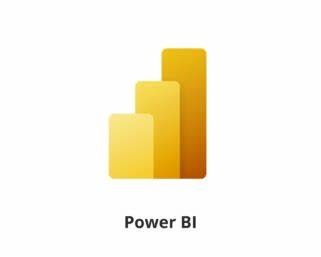
\includegraphics[width=0.18\textwidth]{image/powerbi.jpg} 
\end{center} 
Power BI est un outil de visualisation de données développé par Microsoft. Il permet de créer des rapports interactifs et des tableaux de bord à partir de diverses sources de données. C'est l'outil de visualisation le plus utilisé par la communauté des analystes de données. Son interface facile à utiliser et sa rapidité de création de visualisations m'ont permis de créer des graphiques et des tableaux de bord interactifs pour présenter les résultats de l'analyse des données de manière claire et concise. 

\subsubsection{Microsoft Excel}
\begin{center}
    
\includegraphics[width=0.15\textwidth]{image/excel.png} 
\end{center} 
Excel est un tableur de calcul utilisé pour la manipulation et l'analyse de données. Il est largement utilisé pour des tâches simples de nettoyage, d'agrégation et de visualisation des données. J'ai utilisé Excel pour un petit aperçu des données et faire les premiers filtres pour mieux comprendre les données avant de les importer dans Python pour une analyse plus approfondie. Il m'a permis aussi de faire des filtres et des tableaux croisés dynamiques pour détecter les tendances et les anomalies dans les données. 

\subsubsection{Autres outils} 
D'autres outils et technologies ont été utilisés pour faciliter le travail, notamment :
\begin{itemize}
    \item \textbf{Git} : Pour sauvegarder mon code en ligne et collaborer avec un autre développeur, permettant de suivre les modifications et de gérer les versions du code. 
    \item \textbf{Jupyter Notebook} : Pour le développement interactif et la documentation du code Python, permettant de combiner le code, les visualisations et les explications dans un même document.
    \item \textbf{Slack} : Pour la communication et la collaboration avec l'équipe de la Division des Études Statistiques (DES), facilitant le partage d'informations et la coordination des tâches. 
\end{itemize} 
